\documentclass[xelatex]{beamer}

\title{Xen Hypervisor on Embedded Systems\\~\\\normalsize{Why real folk like it and how we can play video games in the lab}}
\author{Craig Ramsay}
\institute{
  Strathclyde University
}
\date{}

\usepackage{default}
\usepackage[quiet]{fontspec}
\usepackage{xunicode}
\usepackage{xltxtra}
\usepackage{graphicx}
\usepackage{xcolor}
\usepackage{listings}
\usepackage[normalem]{ulem}
\usepackage{amssymb}
\usepackage{ifthen}
\usepackage{tikz}

\frenchspacing
\unitlength=0.01\textwidth
\thicklines
\urlstyle{sf}
\graphicspath{{images/}}

\setsansfont{Open Sans}
\setmonofont{FreeMono}

\setbeamertemplate{frametitle}
  {\begin{centering}\smallskip
   \insertframetitle\par
   \smallskip\end{centering}}
\setbeamertemplate{itemize item}{$\bullet$}
\setbeamertemplate{navigation symbols}{}
\setbeamertemplate{footline}[text line]{%
    \hfill\strut{%
        \scriptsize\sf\color{black!60}%
        \quad\insertframenumber
    }%
    \hfill
}

% Define some colors:
\definecolor{DarkFern}{HTML}{407428}
\definecolor{DarkCharcoal}{HTML}{4D4944}
\colorlet{Fern}{DarkFern!85!white}
\colorlet{Charcoal}{DarkCharcoal!85!white}
\colorlet{LightCharcoal}{Charcoal!50!white}
\colorlet{AlertColor}{orange!80}
\colorlet{DarkRed}{red!70!black}
\colorlet{DarkBlue}{blue!70!black}
\colorlet{DarkGreen}{green!70!black}

\definecolor{StrathBlue}{HTML}{002B5C}
\definecolor{EngBlue}{HTML}{0078AE}
\definecolor{EngBlueLight}{HTML}{68B6D9}
\definecolor{StrathGray}{HTML}{A7A9AC}
% Use the colors:
\setbeamercolor{title}{fg=EngBlue}
\setbeamercolor{frametitle}{fg=EngBlue}
\setbeamercolor{normal text}{fg=Charcoal}
\setbeamercolor{block title}{fg=Charcoal,bg=EngBlueLight!25!white}
\setbeamercolor{block body}{fg=Charcoal,bg=EngBlue!10!white}
\setbeamercolor{alerted text}{fg=AlertColor}
\setbeamercolor{itemize item}{fg=Charcoal}
\setbeamercolor{section in toc}{fg=EngBlue}

\newcommand\titleframe[2][\relax]{
  \begin{frame}[plain]%
    \begin{center}%
      #2
    \end{center}
  \end{frame}
}
\AtBeginSection[]
{
   \begin{frame}[plain]
     \centering
     \begin{beamercolorbox}[sep=8pt,center,shadow=true,rounded=true]{title}
    \usebeamerfont{title}\insertsectionhead\par%
  \end{beamercolorbox}
  ~\\~\\
   \includegraphics[height=0.5\paperheight,width=0.5\paperwidth,keepaspectratio]{\sectionbg}
   \end{frame}
}

%More itemize space
\let\olditem\item
\renewcommand{\item}{%
    \olditem\vspace{12pt}}

%Hide page nums
\setbeamertemplate{footline}[page number]{}
\setbeamertemplate{footline}{}


\begin{document}

\titleframe[substructure]{\titlepage}

\begin{frame}{What is Xen?}
\centering
\vspace*{1.6cm}

\includegraphics[width=0.8\textwidth]{what}
\end{frame}

\begin{frame}[c]{What is Xen?}
\center
\Large
It's a bare-metal hypervisor.
\end{frame}

{
\usebackgroundtemplate{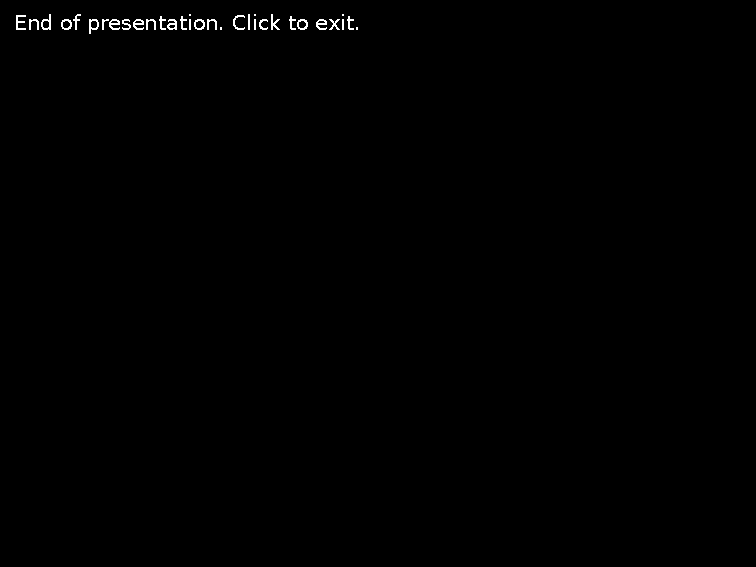
\includegraphics[width=\paperwidth]{end}}
\begin{frame}
\end{frame}
}

\begin{frame}{Really Though\ldots}
\begin{itemize}
\item We use a {\color{blue}hypervisor} to run {\color{green}virtual machines}
\item Xen does this is a neat way
\item Low overhead $\rightarrow$ OK on embedded
\end{itemize}
\end{frame}

\begin{frame}{Traditional Virtualisation}
Hypervisors such as VirtualBox look like this\ldots
\begin{center}
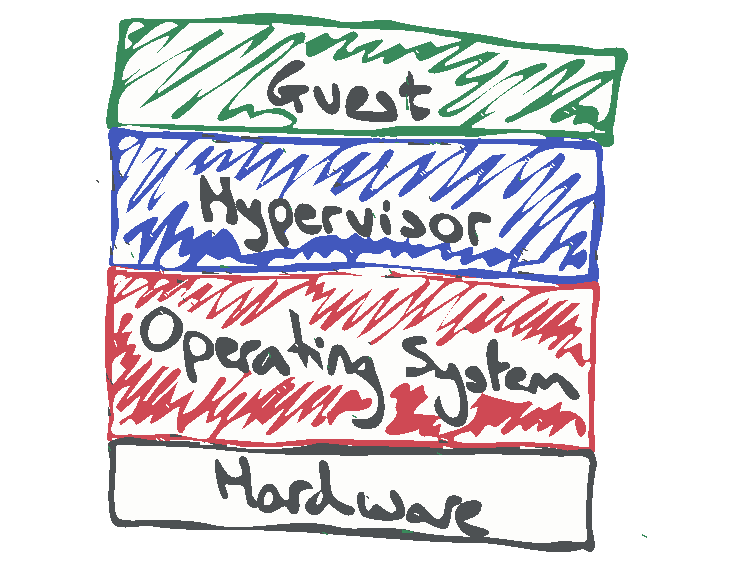
\includegraphics[width=0.7\textwidth]{vbox}
\end{center}
\ldots but less charming
\end{frame}

\begin{frame}{Xen Virtualisation}
Remember "bare-metal" hypervisor?
\\~\\Xen sits on the bare-metal
\begin{center}
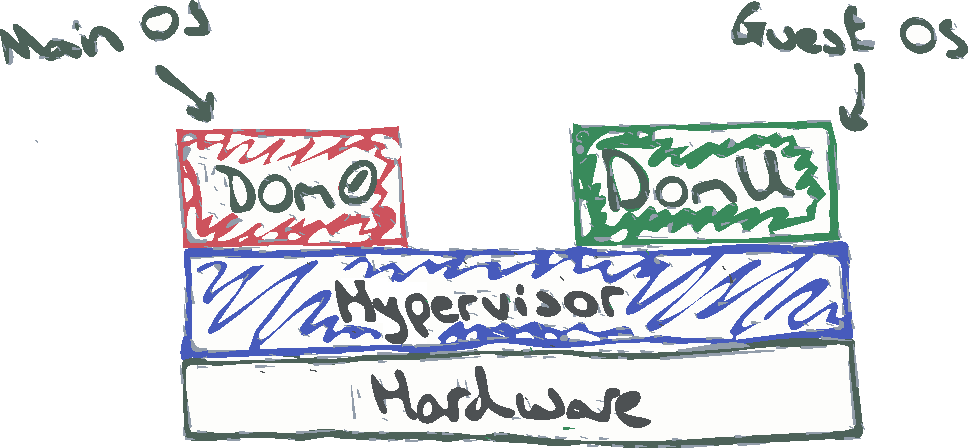
\includegraphics[width=0.9\textwidth]{xen_intro}
\end{center}
\hfill DomU is the guest.\\
Dom $=$ Domain\hfill Dom0 is always needed.
\\TO DO: Clean up these gray bits
\end{frame}

\begin{frame}{Why should I care?}
\begin{itemize}
\item Moore's law $\rightarrow$ Now we can!
\item But why should we?
\end{itemize}
\centering
\input{images/uses.pdf_tex}
\end{frame}

\begin{frame}{How it works: Linux Guests}
\begin{itemize}
\item Dom0 loads totally normal Linux image as a DomU
\begin{itemize}
\item At most, it has Xen aware drivers
\end{itemize}
\item Linux knows it's living a lie
\begin{itemize}
\item {\color{blue}"Paravirtualised"} or {\color{blue}PV}
\end{itemize}
\item Anything hard to virtualise?
\begin{itemize}
\item {Pass it off to Xen via kernel hooks}
\end{itemize}
\item PV gives \emph{much} better performance
\end{itemize}
TO DO: ADD SLIDE WITH EXAMPLE XEN CONF
\end{frame}

\begin{frame}{How it works: Using Hardware}
\begin{itemize}
\item Resource sharing problems!
\begin{itemize}
\item Like parent arbitrating a toy box
\end{itemize}
\item Option to loan device to one guest excusively
\item But some devices need to be shared by many guests!
\begin{itemize}
\item Networking, disk access, etc\ldots
\end{itemize}
\end{itemize}
\end{frame}

\begin{frame}{How it works: Using Hardware}
\begin{itemize}
\item Peripheral is owned by ONE dom but driver is split driver into:
\begin{itemize}
\item "Front" for non-owner to request use
\item "Back" for owner to arbitrate access
\end{itemize}
\end{itemize}
~\\
\centering
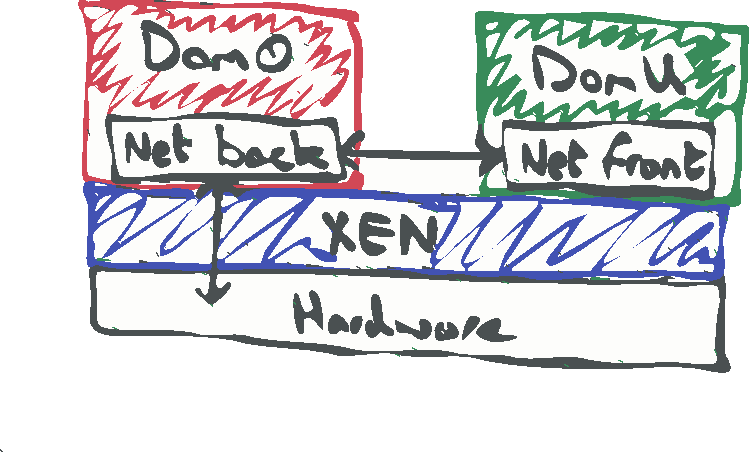
\includegraphics[width=0.8\textwidth]{driver}
\end{frame}

\begin{frame}{How it works: Dumber Guests}
\begin{itemize}
\item Can also run legacy/non-PV guests
\item Usually a euphamism for Windows
\item Fully virtualised via QEMU emulation layer
\end{itemize}
~\\
\centering
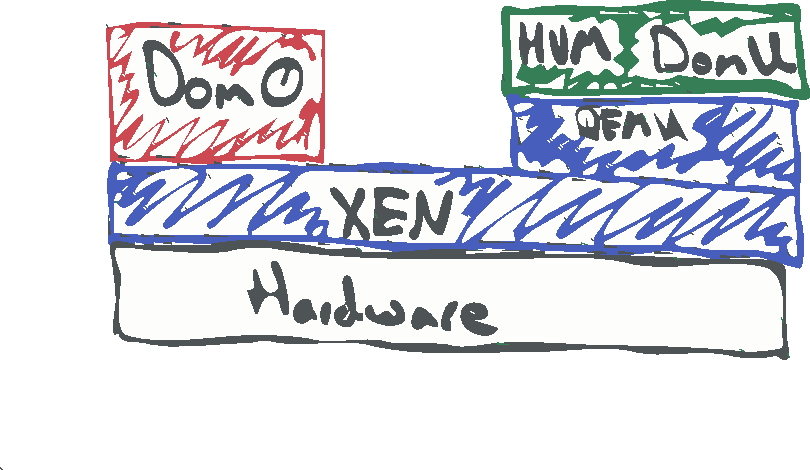
\includegraphics[width=0.8\textwidth]{hvm}
\end{frame}

\begin{frame}{How it works: Scheduling}
\begin{itemize}
\item Can have $>1$ DomU
\item Need to share CPU time
\item Uses "proportional fair share" algorithm:
\begin{itemize}
\item \# virtual CPUs \hfill $=$ mapped to real CPUs
\item weight \hfill $=$ proportional to CPU time
\item cap \hfill $=$ upper limit on CPU time
\end{itemize}
\end{itemize}
\end{frame}

{
\usebackgroundtemplate{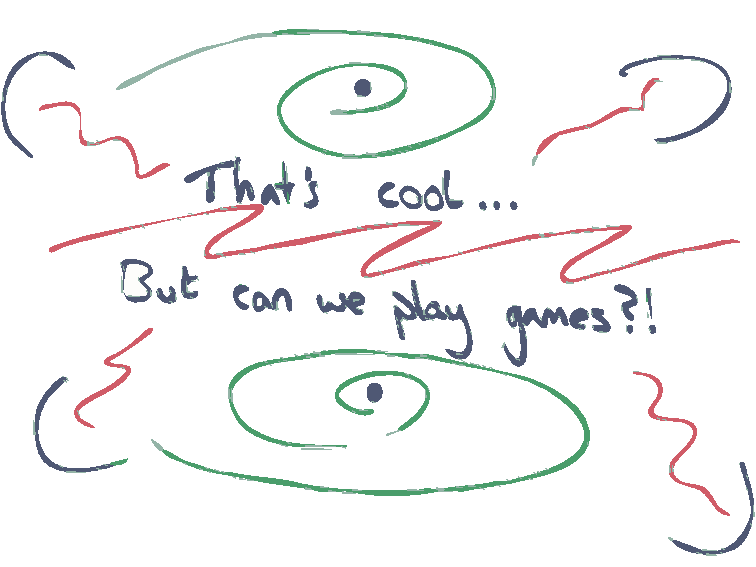
\includegraphics[width=\paperwidth]{games}}
\begin{frame}
\end{frame}
}

\begin{frame}{Demo}
\centering
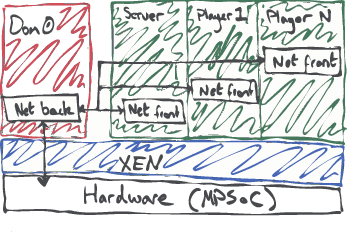
\includegraphics[width=1\textwidth]{demo}
\end{frame}

\begin{frame}{Performance Stigma}
\begin{itemize}
\item "That was cool, but virtualisation is really slow, right?"
\item This laptop is running many XEN VMs right now
\begin{itemize}
\item Including the presentation, for building the demo, Netflix, etc\ldots
\end{itemize}
\end{itemize}
\begin{center}
\vspace{-0.7cm}

\includegraphics[width=\textwidth]{wow}
\end{center}
\vspace{-0.7cm}
\begin{itemize}
\item Paravirtualisation is quite good.
\end{itemize}
\end{frame}

\begin{frame}{Summary}
\begin{itemize}
\item Xen is a bare-metal hypervisor
\item We now know what that means
\item Useful in embedded for app integration, security and resource management
\item Will be important for larger embedded systems
\item Good excuse for some terrible old games!
\end{itemize}
\end{frame}

\end{document}
